%% Преамбула TeX-файла

% 1. Стиль и язык
\documentclass[utf8x,times, 12pt]{G7-32} % Стиль (по умолчанию будет 14pt)

% Остальные стандартные настройки убраны в preamble.inc.tex.
\sloppy

% Настройки стиля ГОСТ 7-32
% Для начала определяем, хотим мы или нет, чтобы рисунки и таблицы нумеровались в пределах раздела, или нам нужна сквозная нумерация.
\EqInChapter % формулы будут нумероваться в пределах раздела
\TableInChapter % таблицы будут нумероваться в пределах раздела
\PicInChapter % рисунки будут нумероваться в пределах раздела

% Добавляем гипертекстовое оглавление в PDF
\usepackage[
bookmarks=true, colorlinks=true, unicode=true,
urlcolor=black,linkcolor=black, anchorcolor=black,
citecolor=black, menucolor=black, filecolor=black,
]{hyperref}

\AfterHyperrefFix

\usepackage{microtype}% полезный пакет для микротипографии, увы под xelatex мало чего умеет, но под pdflatex хорошо улучшает читаемость

% Тире могут быть невидимы в Adobe Reader
\ifInvisibleDashes
\MakeDashesBold
\fi

\usepackage{graphicx}   % Пакет для включения рисунков

% С такими оно полями оно работает по-умолчанию:
% \RequirePackage[left=20mm,right=10mm,top=20mm,bottom=20mm,headsep=0pt,includefoot]{geometry}
% Если вас тошнит от поля в 10мм --- увеличивайте до 20-ти, ну и про переплёт не забывайте:
\geometry{right=20mm}
\geometry{left=30mm}
\geometry{bottom=20mm}
\geometry{ignorefoot}% считать от нижней границы текста


% Пакет Tikz
\usepackage{tikz}
\usetikzlibrary{arrows,positioning,shadows}

% Произвольная нумерация списков.
\usepackage{enumerate}

% ячейки в несколько строчек
\usepackage{multirow}

% itemize внутри tabular
\usepackage{paralist,array}

%\setlength{\parskip}{1ex plus0.5ex minus0.5ex} % разрыв между абзацами
\setlength{\parskip}{1ex} % разрыв между абзацами
\usepackage{blindtext}

% Центрирование подписей к плавающим окружениям
%\usepackage[justification=centering]{caption}

\usepackage{newfloat}
\DeclareFloatingEnvironment[
placement={!ht},
name=Equation
]{eqndescNoIndent}
\edef\fixEqndesc{\noexpand\setlength{\noexpand\parindent}{\the\parindent}\noexpand\setlength{\noexpand\parskip}{\the\parskip}}
\newenvironment{eqndesc}[1][!ht]{%
    \begin{eqndescNoIndent}[#1]%
\fixEqndesc%
}
{\end{eqndescNoIndent}}




\usepackage{pgfplots}
\pgfplotsset{width=\linewidth,compat=1.8}

% Настройки листингов.
\ifPDFTeX
% 8 Листинги

\usepackage{listings}
% \usepackage{listingsutf8}

% Значения по умолчанию
\lstset{
  basicstyle= \footnotesize,
  breakatwhitespace=true,% разрыв строк только на whitespacce
  breaklines=true,       % переносить длинные строки
%   captionpos=b,          % подписи снизу -- вроде не надо
  inputencoding=koi8-r,
  numbers=left,          % нумерация слева
  numberstyle=\footnotesize,
  showspaces=false,      % показывать пробелы подчеркиваниями -- идиотизм 70-х годов
  showstringspaces=false,
  showtabs=false,        % и табы тоже
  stepnumber=1,
  tabsize=4,              % кому нужны табы по 8 символов?
  frame=single
}

% Стиль для псевдокода: строчки обычно короткие, поэтому размер шрифта побольше
\lstdefinestyle{pseudocode}{
  basicstyle=\small,
  keywordstyle=\color{black}\bfseries\underbar,
  language=Pseudocode,
  numberstyle=\footnotesize,
  commentstyle=\footnotesize\it
}

% Стиль для обычного кода: маленький шрифт
\lstdefinestyle{realcode}{
  basicstyle=\scriptsize,
  numberstyle=\footnotesize
}

% Стиль для коротких кусков обычного кода: средний шрифт
\lstdefinestyle{simplecode}{
  basicstyle=\footnotesize,
  numberstyle=\footnotesize
}

% Стиль для BNF
\lstdefinestyle{grammar}{
  basicstyle=\footnotesize,
  numberstyle=\footnotesize,
  stringstyle=\bfseries\ttfamily,
  language=BNF
}

% Определим свой язык для написания псевдокодов на основе Python
\lstdefinelanguage[]{Pseudocode}[]{Python}{
  morekeywords={each,empty,wait,do},% ключевые слова добавлять сюда
  morecomment=[s]{\{}{\}},% комменты {а-ля Pascal} смотрятся нагляднее
  literate=% а сюда добавлять операторы, которые хотите отображать как мат. символы
    {->}{\ensuremath{$\rightarrow$}~}2%
    {<-}{\ensuremath{$\leftarrow$}~}2%
    {:=}{\ensuremath{$\leftarrow$}~}2%
    {<--}{\ensuremath{$\Longleftarrow$}~}2%
}[keywords,comments]

% Свой язык для задания грамматик в BNF
\lstdefinelanguage[]{BNF}[]{}{
  morekeywords={},
  morecomment=[s]{@}{@},
  morestring=[b]",%
  literate=%
    {->}{\ensuremath{$\rightarrow$}~}2%
    {*}{\ensuremath{$^*$}~}2%
    {+}{\ensuremath{$^+$}~}2%
    {|}{\ensuremath{$|$}~}2%
}[keywords,comments,strings]

\lstdefinelanguage[]{MyPs}[]{}{
  morekeywords={each,empty,wait,do},% ключевые слова добавлять сюда
  morecomment=[s]{\{}{\}},
  literate=
    {\\\\}{\ensuremath{$\vartriangleright$}~}2%
    {->}{\ensuremath{$\rightarrow$}~}2%
    {<-}{\ensuremath{$\leftarrow$}~}2%
    {==}{\ensuremath{$=$}~}2%
    {!=}{\ensuremath{$\neq$}~}2%
    {:=}{\ensuremath{$\leftarrow$}~}2%
    {\\in}{\ensuremath{$ \in $}~}2%
    {<--}{\ensuremath{$\Longleftarrow$}~}2%
    {\\times}{\ensuremath{$\times$}~}2%
    {<=}{\ensuremath{$\leq$}~}2%
    {>=}{\ensuremath{$\geq$}~}2%
}[keywords,comments,strings]

% Подписи к листингам на русском языке.
\renewcommand\lstlistingname{Листинг}
\renewcommand\lstlistlistingname{Листинги}



\else
\usepackage{local-minted}
\fi

\usepackage{indentfirst}
\usepackage{ulem} % Нормальное нижнее подчеркивание

% Дополнительное окружения для подписей
\usepackage{array}

\usepackage{svg} 

\usepackage{pdflscape}
% \usepackage{lscape}

% Полезные макросы листингов.
% Любимые команды
\newcommand{\Code}[1]{\textbf{#1}}

\newenvironment{signstabular}[1][1]{
	\renewcommand*{\arraystretch}{#1}
	\tabular
}{
	\endtabular
}



\newcommand{\frc}[2]{\raisebox{2pt}{$#1$}\big/\raisebox{-3pt}{$#2$}}    % a/b, a выше, b ниже

\renewcommand{\labelenumi}{\arabic{enumi})}
\renewcommand{\labelenumii}{\asbuk{enumii})}



\usepackage[T2A]{fontenc} % Поддержка русских букв
% \usepackage[utf8]{inputenc} % Кодировка utf8
% \usepackage[english, russian]{babel} % Языки: русский, английский
% \usepackage{pscyr} % Нормальные шрифты

\usepackage{algorithm}
\usepackage{algpseudocode}
\floatname{algorithm}{Псевдокод}

\algrenewcommand\algorithmicwhile{\textbf{До тех пока}}
\algrenewcommand\algorithmicdo{\textbf{выполнить}}
\algrenewcommand\algorithmicrepeat{\textbf{Повторять}}
\algrenewcommand\algorithmicuntil{\textbf{Пока выполняется}}
\algrenewcommand\algorithmicend{\textbf{Конец}}
\algrenewcommand\algorithmicif{\textbf{Если}}
\algrenewcommand\algorithmicelse{\textbf{иначе}}
\algrenewcommand\algorithmicthen{\textbf{тогда}}
\algrenewcommand\algorithmicfor{\textbf{Цикл}}
\algrenewcommand\algorithmicforall{\textbf{Для всех}}
\algrenewcommand\algorithmicfunction{\textbf{Функция}}
\algrenewcommand\algorithmicprocedure{\textbf{Процедура}}
\algrenewcommand\algorithmicloop{\textbf{Зациклить}}
\algrenewcommand\algorithmicrequire{\textbf{Условия:}}
\algrenewcommand\algorithmicensure{\textbf{Обеспечивающие условия:}}
\algrenewcommand\algorithmicreturn{\textbf{Возвратить}}
\algrenewtext{EndWhile}{\textbf{Конец цикла}}
\algrenewtext{EndLoop}{\textbf{Конец зацикливания}}
\algrenewtext{EndFor}{\textbf{Конец цикла}}
\algrenewtext{EndFunction}{\textbf{Конец функции}}
\algrenewtext{EndProcedure}{\textbf{Конец процедуры}}
\algrenewtext{EndIf}{\textbf{Конец условия}}
\algrenewtext{EndFor}{\textbf{Конец цикла}}
\algrenewtext{BeginAlgorithm}{\textbf{Начало алгоритма}}
\algrenewtext{EndAlgorithm}{\textbf{Конец алгоритма}}
\algrenewtext{BeginBlock}{\textbf{Начало блока. }}
\algrenewtext{EndBlock}{\textbf{Конец блока}}
\algrenewtext{ElsIf}{\textbf{иначе если }}

\renewcommand{\thealgorithm}{\thechapter.\arabic{algorithm}}%

\makeatletter
\@addtoreset{algorithm}{chapter}% algorithm counter resets every chapter
\makeatother



% Fix breaking algos per page 
\makeatletter
\newenvironment{breakablealgorithm}
  {% \begin{breakablealgorithm}
   \begin{center}
     \refstepcounter{algorithm}% New algorithm
     \hrule height.8pt depth0pt \kern2pt% \@fs@pre for \@fs@ruled
     \renewcommand{\caption}[2][\relax]{% Make a new \caption
       {\raggedright\textbf{\fname@algorithm~\thealgorithm} ##2\par}%
       \ifx\relax##1\relax % #1 is \relax
         \addcontentsline{loa}{algorithm}{\protect\numberline{\thealgorithm}##2}%
       \else % #1 is not \relax
         \addcontentsline{loa}{algorithm}{\protect\numberline{\thealgorithm}##1}%
       \fi
       \kern2pt\hrule\kern2pt
     }
  }{% \end{breakablealgorithm}
     \kern2pt\hrule\relax% \@fs@post for \@fs@ruled
   \end{center}
  }
\makeatother



\addto\captionsrussian{%
 \def\contentsname{%
  Содержание}%
 \def\bibname{%
  Список~
  литературы}%
}

\begin{document}

\frontmatter % выключает нумерацию ВСЕГО; здесь начинаются ненумерованные главы: реферат, введение, глоссарий, сокращения и прочее.

\begin{titlepage}
    \thispagestyle{empty}

    \noindent\begin{minipage}{0.05\textwidth}
        
\includegraphics[scale=0.3]{img/bmstu.png}
    \end{minipage}
    \hfill
    \begin{minipage}{0.85\textwidth}\raggedleft
        \begin{center}
            \fontsize{12pt}{0.3\baselineskip}\selectfont \textbf{Министерство науки и высшего образования Российской Федерации \\ Федеральное государственное бюджетное образовательное учреждение \\ высшего образования \\ <<Московский государственный технический университет \\ имени Н.Э. Баумана \\ (национальный исследовательский университет)>> \\ (МГТУ им. Н.Э. Баумана)}
        \end{center}
    \end{minipage}

    \begin{center}
        \fontsize{12pt}{0.1\baselineskip}\selectfont
        \noindent\makebox[\linewidth]{\rule{\textwidth}{4pt}} \makebox[\linewidth]{\rule{\textwidth}{1pt}}
    \end{center}

    \begin{flushleft}
        \fontsize{12pt}{0.8\baselineskip}\selectfont

        ФАКУЛЬТЕТ \uline{
            Информатика и системы управления
            \hfill}

        КАФЕДРА \uline{\mbox{\hspace{4mm}}
            Программное обеспечение ЭВМ и информационные технологии
            \hfill}
    \end{flushleft}

    \vfill

    \begin{center}
        \fontsize{20pt}{\baselineskip}\selectfont

        \textbf{ОТЧЕТ \\ по лабораторной работе №6}
    \end{center}



    \vfill
    \begin{table}[h!]
        \fontsize{14pt}{0.7\baselineskip}\selectfont
        % \centering
        \begin{signstabular}[0.7]{p{3cm} >{\centering\arraybackslash}p{12.5cm} >{\centering\arraybackslash}p{4cm}}
            Название: & \uline{\hfill Муравьиный алгоритм \hfill}
        \end{signstabular}

        \vspace{\baselineskip}

        \begin{signstabular}[0.7]{p{3cm} >{\centering\arraybackslash}p{12.5cm} >{\centering\arraybackslash}p{4cm}}
            Дисциплина: & \uline{\hfill Анализ алгоритмов \hfill}
        \end{signstabular}

        \vspace{\baselineskip}


    \end{table}
    \vfill

    \begin{table}[h!]
        \fontsize{14pt}{0.7\baselineskip}\selectfont
        % \centering
        \begin{signstabular}[0.7]{p{3cm} >{\centering\arraybackslash}p{2cm}>{\centering\arraybackslash}p{1cm} >{\centering\arraybackslash}p{4cm} >{\centering\arraybackslash}p{4cm}}
            Студент & \uline{\hfill ИУ7-54б \hfill } && \uline{\mbox{\hspace*{4cm}}} & \uline{\hfill  Ларин В.Н. \hfill} \\
            &\scriptsize (группа)&& \scriptsize (подпись, дата) & \scriptsize (фамилия, и.о.)
        \end{signstabular}

        \vspace{\baselineskip}

        \begin{signstabular}[0.7]{p{3cm} >{\centering\arraybackslash}p{2cm}>{\centering\arraybackslash}p{1cm} >{\centering\arraybackslash}p{4cm} >{\centering\arraybackslash}p{4cm}}
            Преподаватель &&&  \uline{\mbox{\hspace*{4cm}}} & \uline{\hfill Волкова Л.Л. \hfill} \\
            &&& \scriptsize (подпись, дата) & \scriptsize (фамилия, и.о.)
        \end{signstabular}
        \vspace{\baselineskip}
        \vspace{\baselineskip}

    \end{table}

    \vfill

    \begin{center}
        \normalsize \textbf{Москва, 2021} 
    \end{center}
\end{titlepage}



% \begin{executors}
% \personalSignature{Первый исполнитель}{ФИО}

% \personalSignature{Второй исполнитель}{ФИО}
% \end{executors}


%\listoffigures                         % Список рисунков

%\listoftables                          % Список таблиц

%\NormRefs % Нормативные ссылки 
% Команды \breakingbeforechapters и \nonbreakingbeforechapters
% управляют разрывом страницы перед главами.
% По-умолчанию страница разрывается.

% \nobreakingbeforechapters
% \breakingbeforechapters



% \begin{titlepage}
    \thispagestyle{empty}

    \noindent\begin{minipage}{0.05\textwidth}
        
\includegraphics[scale=0.3]{img/bmstu.png}
    \end{minipage}
    \hfill
    \begin{minipage}{0.85\textwidth}\raggedleft
        \begin{center}
            \fontsize{12pt}{0.3\baselineskip}\selectfont \textbf{Министерство науки и высшего образования Российской Федерации \\ Федеральное государственное бюджетное образовательное учреждение \\ высшего образования \\ <<Московский государственный технический университет \\ имени Н.Э. Баумана \\ (национальный исследовательский университет)>> \\ (МГТУ им. Н.Э. Баумана)}
        \end{center}
    \end{minipage}

    \begin{center}
        \fontsize{12pt}{0.1\baselineskip}\selectfont
        \noindent\makebox[\linewidth]{\rule{\textwidth}{4pt}} \makebox[\linewidth]{\rule{\textwidth}{1pt}}
    \end{center}

    \begin{flushleft}
        \fontsize{12pt}{0.8\baselineskip}\selectfont

        ФАКУЛЬТЕТ \uline{
            Информатика и системы управления
            \hfill}

        КАФЕДРА \uline{\mbox{\hspace{4mm}}
            Программное обеспечение ЭВМ и информационные технологии
            \hfill}
    \end{flushleft}

    \vfill

    \begin{center}
        \fontsize{20pt}{\baselineskip}\selectfont

        \textbf{ОТЧЕТ \\ по лабораторной работе №6}
    \end{center}



    \vfill
    \begin{table}[h!]
        \fontsize{14pt}{0.7\baselineskip}\selectfont
        % \centering
        \begin{signstabular}[0.7]{p{3cm} >{\centering\arraybackslash}p{12.5cm} >{\centering\arraybackslash}p{4cm}}
            Название: & \uline{\hfill Муравьиный алгоритм \hfill}
        \end{signstabular}

        \vspace{\baselineskip}

        \begin{signstabular}[0.7]{p{3cm} >{\centering\arraybackslash}p{12.5cm} >{\centering\arraybackslash}p{4cm}}
            Дисциплина: & \uline{\hfill Анализ алгоритмов \hfill}
        \end{signstabular}

        \vspace{\baselineskip}


    \end{table}
    \vfill

    \begin{table}[h!]
        \fontsize{14pt}{0.7\baselineskip}\selectfont
        % \centering
        \begin{signstabular}[0.7]{p{3cm} >{\centering\arraybackslash}p{2cm}>{\centering\arraybackslash}p{1cm} >{\centering\arraybackslash}p{4cm} >{\centering\arraybackslash}p{4cm}}
            Студент & \uline{\hfill ИУ7-54б \hfill } && \uline{\mbox{\hspace*{4cm}}} & \uline{\hfill  Ларин В.Н. \hfill} \\
            &\scriptsize (группа)&& \scriptsize (подпись, дата) & \scriptsize (фамилия, и.о.)
        \end{signstabular}

        \vspace{\baselineskip}

        \begin{signstabular}[0.7]{p{3cm} >{\centering\arraybackslash}p{2cm}>{\centering\arraybackslash}p{1cm} >{\centering\arraybackslash}p{4cm} >{\centering\arraybackslash}p{4cm}}
            Преподаватель &&&  \uline{\mbox{\hspace*{4cm}}} & \uline{\hfill Волкова Л.Л. \hfill} \\
            &&& \scriptsize (подпись, дата) & \scriptsize (фамилия, и.о.)
        \end{signstabular}
        \vspace{\baselineskip}
        \vspace{\baselineskip}

    \end{table}

    \vfill

    \begin{center}
        \normalsize \textbf{Москва, 2021} 
    \end{center}
\end{titlepage}

\pagenumbering{gobble}

\tableofcontents


\printnomenclature % Автоматический список сокращений


\Introduction

\pagenumbering{arabic}
\setcounter{page}{2}


Задача поиска оптимальных маршрутов является одной из важных.
Муравьиный алгоритм – один из эффективных полиномиальных алгоритмов для нахождения приближённых решений задачи коммивояжёра, а также решения аналогичных задач поиска маршрутов на графах. Суть подхода заключается в анализе и использовании модели поведения муравьёв, ищущих пути от колонии к источнику питания, и представляет собой метаэвристическую оптимизацию.

Целью данной лабораторной работы является изучение муравьиного алгоритма на примере задачи коммивояжера.

Для достижения поставленной цели необходимо выполнить следующие задачи:

\begin{itemize}
	\item исследовать задачу коммивояжера;
	\item изучить алгоритм полного перебора и муравьиный алгоритм для решения задачи коммивояжера;
	\item провести параметризацию муравьиного алгоритма на двух классах данных;
	\item привести схемы используемых алгоритмов;
	\item описать используемые структуры данных;
	\item описать структуру разрабатываемого ПО;
	\item определить средства программной реализации;
	\item провести сравнительный анализ времени работы алгоритмов;
	\item провести функциональное тестирование;
	\item описать и обосновать полученные результаты в отчете о выполненной лабораторной работе.
\end{itemize}







\mainmatter % это включает нумерацию глав и секций в документе ниже

\chapter{Аналитический раздел}\label{analyth}

\section{Сортировка пузырьком}

Алгоритм состоит из повторяющихся проходов по сортируемому массиву. За каждый проход элементы последовательно сравниваются попарно и если порядок в паре неверный (возрастание, в случае сортировки по убыванию, и наоборот), выполняется обмен элементов. Проходы по массиву повторяются $N−1$ раз \cite{knut}.  

Также существует модифицированная версия данного алгоритма: добавляется флаг, которые показывает были ли обмены в данном цикле. Данный флаг показывает отсортирован ли массив.

\section{Сортировка вставками}

Сортировка вставками — алгоритм сортировки, в котором элементы входной последовательности просматриваются по одному, и каждый новый поступивший элемент размещается в подходящее место среди ранее упорядоченных элементов \cite{knut}.

Массив условно делится на две части: отсортированную и требующую сортировки. В начальный момент отсортированная последовательность пуста. На каждом шаге алгоритма выбирается один из элементов входных данных и помещается на нужную позицию в уже отсортированной последовательности до тех пор, пока набор входных данных не будет исчерпан. В любой момент времени в отсортированной последовательности элементы удовлетворяют требованиям к выходным данным алгоритма

\section{Сортировка выбором}

Существует семейство сортировок, основанное на идее многократного выбора. Простейшая сортировка, основанная на следующей идее. Массив условно делится на две части: отсортированную и требующую сортировки \cite{knut}.
Из правой части выбирается наименьший элемент и добавляется в конец отсортированной части с помощью обмена первого элемента не отсортированной части и минимального данной части.

\section{Требование к ПО}

Программа должна отвечать следующем требованиям:
\begin{enumerate}
	\item На вход подается длинна массива и массив чисел разделенные пробельным символом;
	\item ПО должно выводить отсортированный массив.
\end{enumerate}

\section{Вывод}
В данной работе стоит задача реализации 3 алгоритмов сортировки, а именно: пузырьком, вставками и выбором. Необходимо оценить трудоемкость алгоритмов и проверить ее экспериментально.
\chapter{Конструкторский раздел}
\label{cha:design}

В данном разделе будут приведены схемы конвейерной и линейной реализаций алгоритмов обработки матриц, приведено описание используемых типов данных, а также описана структура ПО.

\section{Схемы алгоритмов}

На рис. \ref{fig:linear_processing} - \ref{fig:stages} приведены схемы линейной и конвейерной реализаций алгоритмов обработки матрицы, схема трёх лент для конвейерной обработки матрицы, а также схемы реализаций этапов обработки матроицы.


\begin{figure}[h]
	\centering
	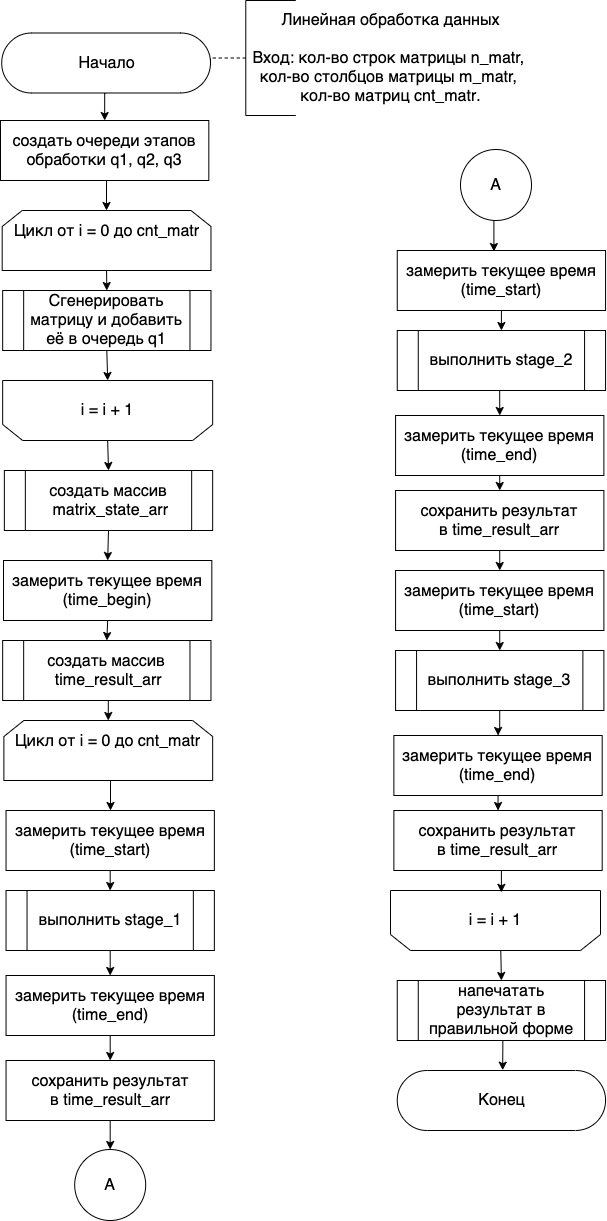
\includegraphics[scale=0.55]{img/linear_processing.png}
	\caption{Схема алгоритма линейной обработки матроицы}
	\label{fig:linear_processing}
\end{figure}

\clearpage

\begin{figure}[h]
	\centering
	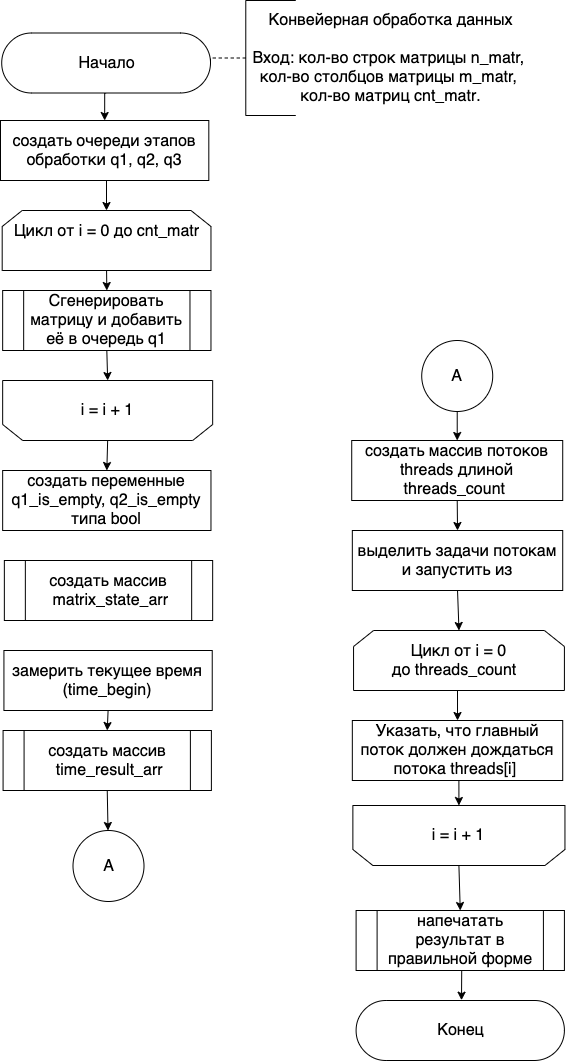
\includegraphics[scale=0.6]{img/parallel_processing.png}
	\caption{Схема алгоритма конвейерной обработки матроицы}
	\label{fig:parallel_processing}
\end{figure}

\clearpage

\begin{figure}[h]
	\centering
	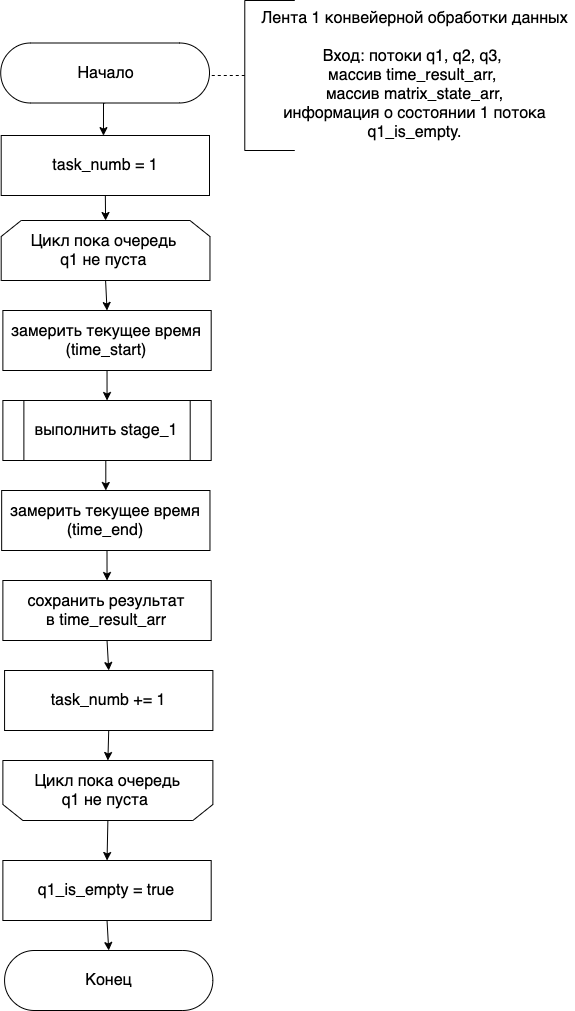
\includegraphics[scale=0.6]{img/parallel_stage_1.png}
	\caption{Схема 1-ой ленты конвейерной обработки матрицы}
	\label{fig:parallel_stage_1}
\end{figure} 

\clearpage

\begin{figure}[h]
	\centering
	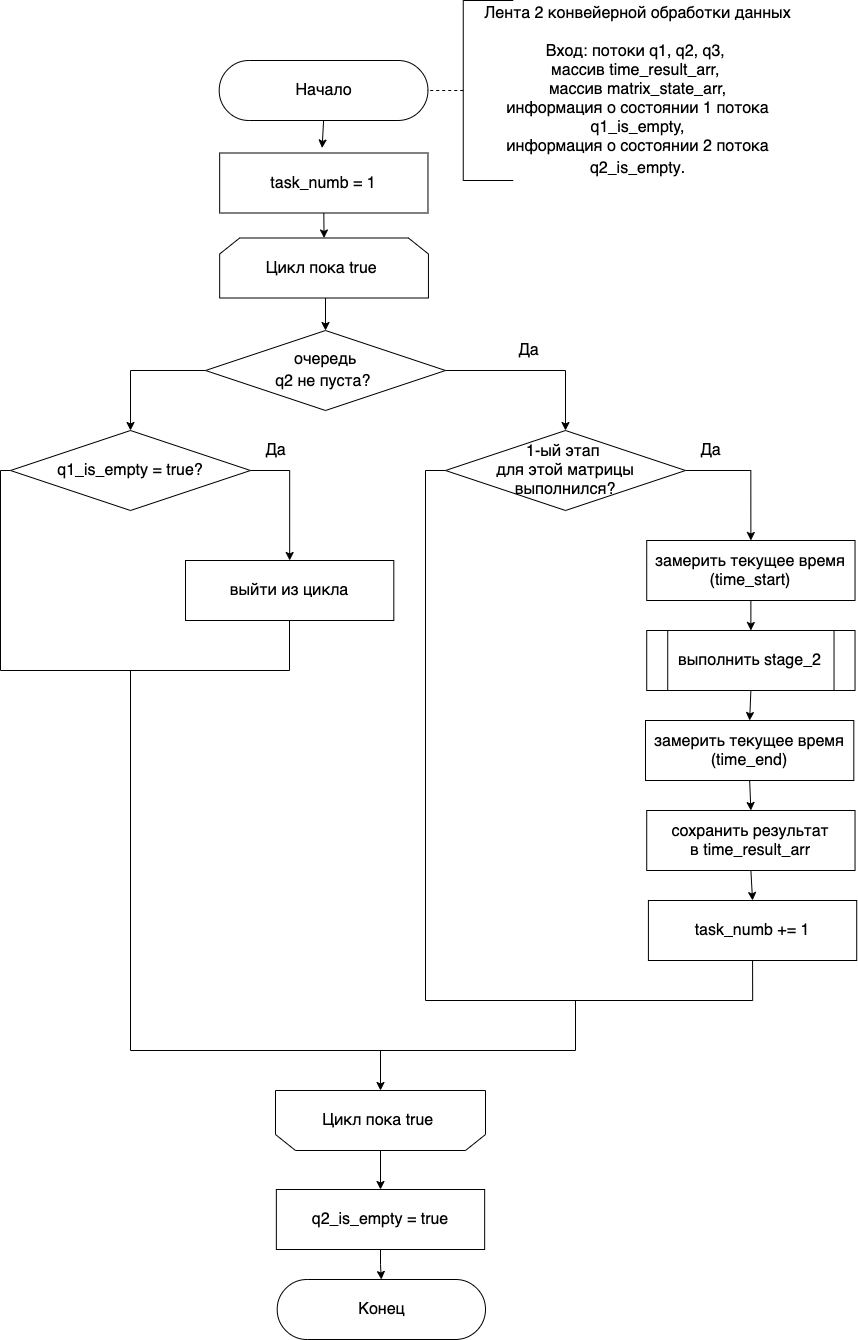
\includegraphics[scale=0.5]{img/parallel_stage_2.png}
	\caption{Схема 2-ой ленты конвейерной обработки матрицы}
	\label{fig:parallel_stage_2}
\end{figure} 

\clearpage

\begin{figure}[h]
	\centering
	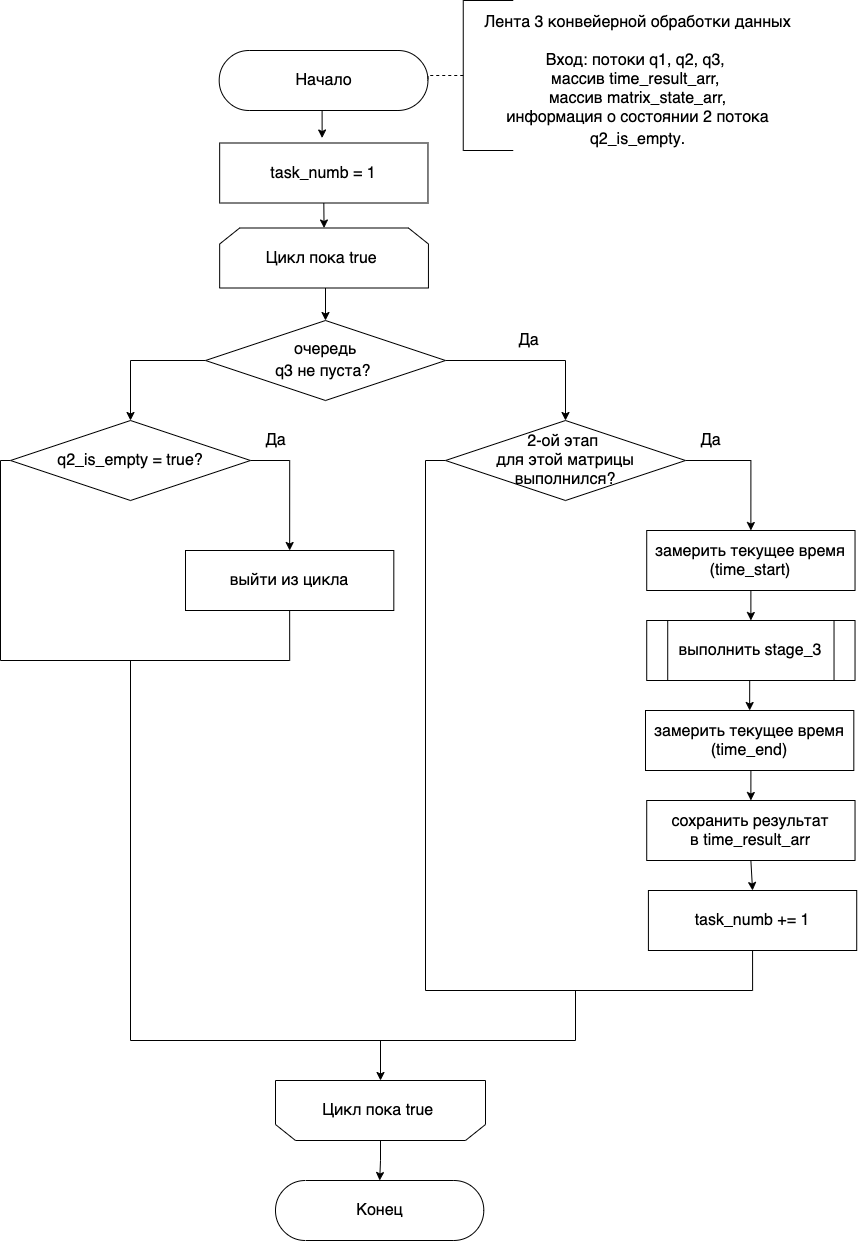
\includegraphics[scale=0.5]{img/parallel_stage_3.png}
	\caption{Схема 3-ей ленты конвейерной обработки матрицы}
	\label{fig:parallel_stage_3}
\end{figure} 

\clearpage

\begin{figure}[h]
	\centering
	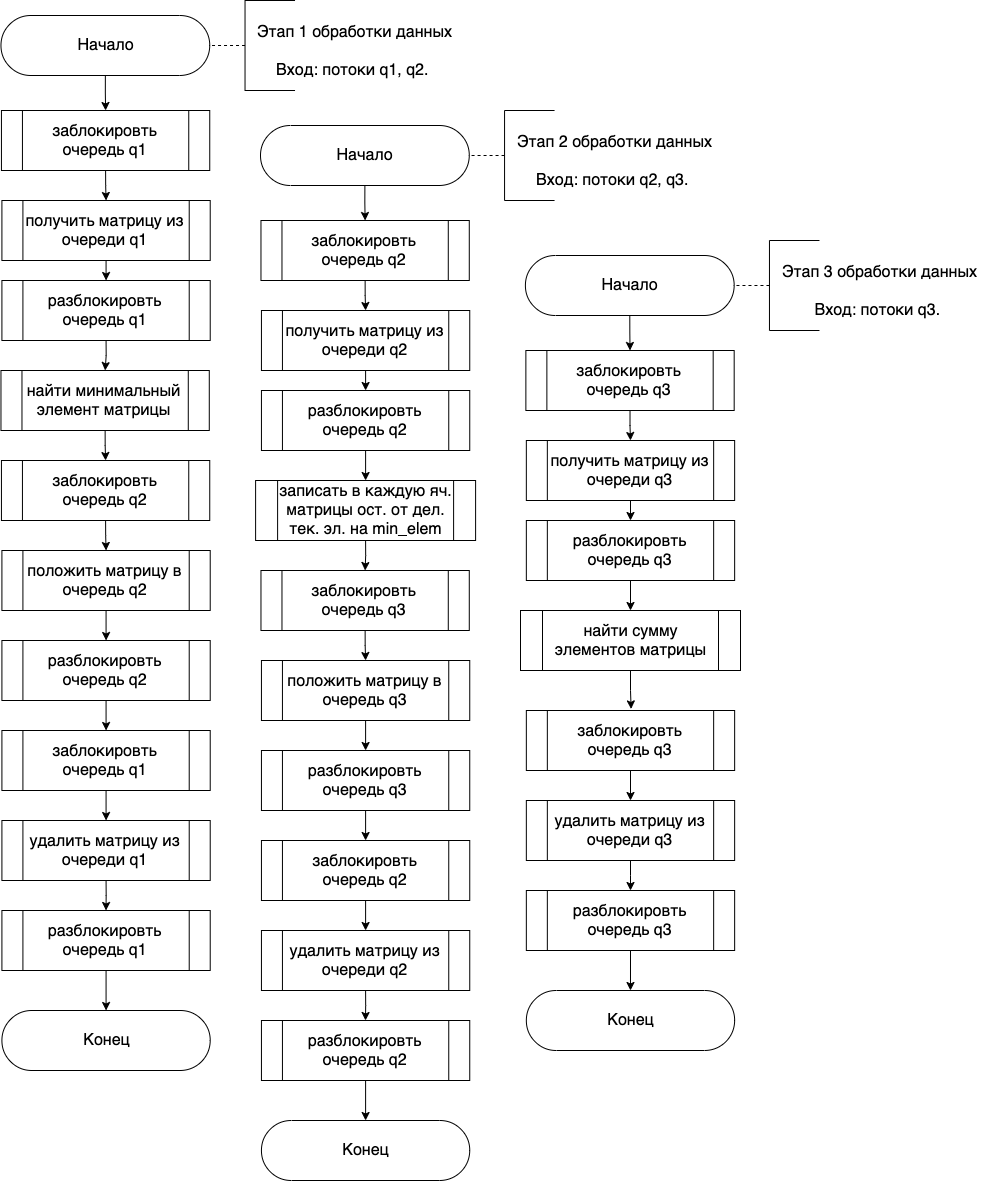
\includegraphics[scale=0.5]{img/stages.png}
	\caption{Схема реализаций этапов обработки матроицы}
	\label{fig:stages}
\end{figure} 

\clearpage

\section{Классы эквивалентности}

Выделенные классы эквивалентности для тестирования:

\begin{itemize}
	\item количество строк матрицы <= 0;
	\item количество столбцов матрицы <= 0;
	\item количество строк матрицы не является целым числом;
	\item количество столбцов матрицы не является целым числом;
	\item количество обрабатываемых матриц <= 0;
	\item количество обрабатываемых матриц не является целым числом;
	\item номер команды < 0 или > 3;
	\item номер команды не является целым числом;
	\item корректный ввод всех параметров;
\end{itemize}

\clearpage

\section{Структура ПО}

ПО будет состоять из следующих модулей:

\begin{itemize}
	\item main.cpp -- файл, содержащий функцию main;
    \item matrix.cpp -- файл, содержащий функции для работы с матрицей;
    \item compare.cpp -- файл, в котором содержатся функции для замера времени работы алгоритмов;
    \item read.cpp -- файл, в котором содержатся функции ввода данных;
    \item conveyor.cpp -- файл, в котором содержатся функции для конвейерной и линейной обработок матриц;
\end{itemize}

\section{Вывод}

В данном разделе на основе теоретических данных были построены схемы требуемых методов обработки матриц (конвейерного и линейного), выбраны используемые типы данных, выделены классы эквивалентности для тестирования, а также была описана структура ПО.

%%% Local Variables:
%%% mode: latex
%%% TeX-master: "rpz"
%%% End:

\chapter{Технологический раздел}
\label{cha:impl}



В данном разделе будут приведены средства реализации, листинги кода, а также функциональные тесты.


\section{Средства реализации}

Основным средством разработки является язык программирования. Был выбран язык программирования C++. Данный выбор обоснован высокой скоростью работы языка, поддержкой строгой типизации \cite{cpplang}. Для сборки проекта был выбран инструмент CMake \cite{cmake}.  В качестве среды разработки был выбран инструмент JetBrains Clion \cite{clion}.


\section{Листинги кода}

В листингах \ref{lst:parallel_processing} - \ref{lst:stage_3} представлены функции для конвейерного и линейного алгоритмов обработки матриц.

\lstinputlisting[language=c,caption={Функция алгоритма конвейерной обработки матриц},label=lst:parallel_processing]{code/conveyor.cpp}
\lstinputlisting[language=c,caption={Функция алгоритма линейной обработки матрицы},label=lst:linear_processing]{code/linear.cpp}

\lstinputlisting[language=c,caption={Функция 1-ой ленты конвейерной обработки матрицы},label=lst:parallel_stage_1]{code/parallel_stage_1.cpp}
\lstinputlisting[language=c,caption={Функция 2-ой ленты конвейерной обработки матрицы},label=lst:parallel_stage_2]{code/parallel_stage_2.cpp}
\lstinputlisting[language=c,caption={Функция 3-ой ленты конвейерной обработки матрицы},label=lst:parallel_stage_3]{code/parallel_stage_3.cpp}

\lstinputlisting[language=c,caption={Функция реализации 1-ого этапа обработки матрицы},label=lst:stage_1]{code/stage_1.cpp}
\lstinputlisting[language=c,caption={Функция реализации 2-ого этапа обработки матрицы},label=lst:stage_2]{code/stage_2.cpp}
\lstinputlisting[language=c,caption={Функция реализации 3-ого этапа обработки матрицы},label=lst:stage_3]{code/stage_3.cpp}


\section{Функциональные тесты}

В таблице \ref{tbl:functional_test} приведены функциональные тесты для конвейерного и ленейного алгоритмов обработки матриц. Все тесты пройдены успешно.

\begin{table}[h]
	\begin{center}
	% \begin{threeparttable}
		\captionsetup{justification=raggedright,singlelinecheck=off}
		\caption{\label{tbl:functional_test} Функциональные тесты}
		\begin{tabular}{|c|c|c|c|c|}
			\hline
			Строк & Столбцов & Метод обр. & Алгоритм & Ожидаемый результат 
			\\ \hline
			0 & 10 & 10 & Конвейерный & Сообщение об ошибке 
			\\ \hline
			k & 10 & 10 & Конвейерный & Сообщение об ошибке 
			\\ \hline
			10 & 0 & 10 & Конвейерный & Сообщение об ошибке 
			\\ \hline
			10 & k & 10 & Конвейерный & Сообщение об ошибке 
			\\ \hline
			10 & 10 & -5 & Конвейерный & Сообщение об ошибке 
			\\ \hline
			10 & 10 & k & Конвейерный & Сообщение об ошибке 
			\\ \hline
			100 & 100 & 20 & Конвейерный & Вывод результ. таблички
			\\ \hline
			100 & 100 & 20 & Линейный & Вывод результ. таблички
			\\ \hline
			50 & 100 & 100 & Линейный & Вывод результ. таблички
			\\ \hline
		\end{tabular}
	% \end{threeparttable}
	\end{center}
\end{table}

\section{Вывод}

В данном разделе были разработаны алгоритмы для конвейерного и ленейного алгоритмов обработки матриц, проведено тестирование, описаны средства реализации и требования к ПО.


\chapter{Экспериментальный раздел}
\label{cha:research}

\section{Технические характеристики}
Тестирование выполнялось на устройстве со следующими техническими характеристиками:
\begin{itemize}
	\item Операционная система Ubuntu 21.04;
	\item Память 16 GiB (4,5 GiB выделено для нужд графического ядра)
	\item Процессор AMD® Ryzen 5 5500u with radeon graphics × 12 
\end{itemize}

\section{Время выполнения алгоритмов}

Для замеров времени использовалась стандартная функция языка clock \cite{clock}.  Данная функция возвращает суммарное процессорное время, использованное программой. В случае ошибки, функция возвращает значение -1. На листинге \ref{listing:mesuare} показан способ применения данной функции при замерах.

\begin{lstlisting}[caption={Замер времени функции}, label=listing:mesuare]
auto start = clock();
for (int j = 0; j < counts; ++j) {
    rec_l(left, right);
}
res.rl = double(clock() - start) / counts;
\end{lstlisting}


Результаты тестирования приведены в таблице \ref{tbl:time} .Прочерк в таблице означает что тестирование для этого набора данных не выполнялось.

\begin{table}[h]
    \caption{Таблица зависимости времени работы реализаций алгоритмов от длины входных слов}
    \begin{tabular}{||l|llll||}
    \hline
    Длина слов & \begin{tabular}[c]{@{}l@{}}Рекурсивный\\ Левенштейна\end{tabular} & \begin{tabular}[c]{@{}l@{}}Итеративный\\ Левенштейна\end{tabular} & \begin{tabular}[c]{@{}l@{}}Рекурсивный с кэшем\\ Левенштейна\end{tabular} & \begin{tabular}[c]{@{}l@{}}Рекурсивный\\ Дамерау--Левенштейна\end{tabular} \\ \hline \hline
    1          & 0.5                                                               & 0.3                                                               & 0.5                                                                       & 0.7                                                                        \\ \hline
    2          & 0.2                                                               & 0.4                                                               & 0.5                                                                       & 1.3                                                                        \\ \hline
    3          & 0.9                                                               & 0.6                                                               & 0.7                                                                       & 6.7                                                                        \\ \hline
    4          & 4.6                                                               & 0.8                                                               & 1.1                                                                       & 34.4                                                                       \\ \hline
    5          & 23.8                                                              & 1                                                                 & 1.5                                                                       & 183.9                                                                      \\ \hline
    6          & 127.6                                                             & 1.3                                                               & 2.1                                                                       & 961.9                                                                      \\ \hline
    7          & 689.6                                                             & 1.7                                                               & 3.2                                                                       & 4756.3                                                                     \\ \hline
    8          & 3488.9                                                            & 2.8                                                               & 6.7                                                                       & 34719.2                                                                    \\ \hline
    9          & 23001.5                                                           & 2.4                                                               & 4.9                                                                       & 145662                                                                     \\ \hline
    10         & 111428                                                            & 3                                                                 & 5.9                                                                       & 797734                                                                     \\ \hline
    20         & --                                                                & 10.3                                                              & 22.5                                                                      & --                                                                         \\ \hline
    30         & --                                                                & 22.5                                                              & 46.1                                                                      & --                                                                         \\ \hline
    50         & --                                                                & 59.9                                                              & 132.8                                                                     & --                                                                         \\ \hline
    100        & --                                                                & 236.4                                                             & 530.1                                                                     & --                                                                         \\ \hline
    200        & --                                                                & 921                                                               & 2047.2                                                                    & --                                                                         \\ \hline
    \end{tabular}
    \label{tbl:time}
    \end{table}

Представлены зависимости времени работы рекурсивных алгоритмов Левенштейна и Дамерау--Левенштейна на рисунках \ref{fig:plot_rec_l} и \ref{fig:plot_rec_e}

\begin{figure}[h]
    \centering
    
    \begin{tikzpicture}
        \begin{axis} [
            legend pos = north west, 
            ymin = 0, 
            grid = major,
            xlabel={Длина слов},
            ylabel={Количество тиков},
            table/col sep = semicolon,
            /pgf/number format/1000 sep={}
        ]
        \legend{ 
            Рекурсивный алгоритм Дамерау-Левенштейна, 
            Рекурсивный алгоритм Левенштейна
        };
        \addplot table [x=x, y=y] {bench_results/dl.csv};
        \addplot table [x=x, y=y] {bench_results/rl.csv};
        \end{axis}
    \end{tikzpicture}

    \caption{Зависимость времени работы реализаций рекурсивных алгоритмов Левенштейна и Дамерау-Левенштейна от времени}
    \label{fig:plot_rec_l}
\end{figure} 


\begin{figure}[h]
    \centering
    
    \begin{tikzpicture}
        \begin{semilogyaxis} [
            legend pos = north west, 
            ymin = 0,
            grid = major,
            xlabel={Длина слов},
            ylabel={Количество тиков},
            table/col sep = semicolon,
            /pgf/number format/1000 sep={}
        ]
        \legend{ 
            Рекурсивный алгоритм Дамерау-Левенштейна, 
            Рекурсивный алгоритм Левенштейна
        };
        \addplot table [x=x, y=y] {bench_results/dl.csv};
        \addplot table [x=x, y=y] {bench_results/rl.csv};
        \end{semilogyaxis}
    \end{tikzpicture}

    \caption{Зависимость времени работы реализаций рекурсивных алгоритмов Левенштейна и Дамерау-Левенштейна от времени в логарифмической шкале}
    
    \label{fig:plot_rec_e}
\end{figure} 

На рисунках \ref{fig:plot_iter_1} и \ref{fig:plot_iter_2} представлена зависимость времени работы реализаций алгоритмов Левенштейна итеративного и рекурсивного с кэшем. 

\begin{figure}[h]
    \centering
    
    \begin{tikzpicture}
        \begin{axis} [
            legend pos = north west, 
            ymin = 0, 
            grid = major,
            xlabel={Длина слов},
            ylabel={Количество тиков},
            table/col sep = semicolon,
            /pgf/number format/1000 sep={}
        ]
        \legend{ 
            Итеративный алгоритм Левенштейна, 
            Рекурсивный алгоритм Левенштейна с кэшированием
        };
        \addplot table [x=x, y=y] {bench_results/il.csv};
        \addplot table [x=x, y=y] {bench_results/rcl.csv};
        \end{axis}
    \end{tikzpicture}

    \caption{Зависимость времени работы реализаций алгоритмов Левенштейна итеративного и рекурсивного с кэшем}
    
    \label{fig:plot_iter_1}
\end{figure} 


\begin{figure}[h]
    \centering
    
    \begin{tikzpicture}
        \begin{axis} [
            legend pos = north west, 
            ymin = 0, 
            grid = major,
            xlabel={Длина слов},
            ylabel={Количество тиков},
            table/col sep = semicolon,
            /pgf/number format/1000 sep={}
        ]
        \legend{ 
            Итеративный алгоритм Левенштейна, 
            Рекурсивный алгоритм Левенштейна с кэшированием
        };
        \addplot table [x=x, y=y] {bench_results/il2.csv};
        \addplot table [x=x, y=y] {bench_results/rcl2.csv};
        \end{axis}
    \end{tikzpicture}

    \caption{Зависимость времени работы реализаций алгоритмов Левенштейна итеративного и рекурсивного с кэшем}
    
    \label{fig:plot_iter_2}
\end{figure} 

\section{Использование памяти}

Максимальная глубина стека при вызове рекурсивных функций рассчитывается по формуле \eqref{eq:rec-mem}.

\begin{eqndesc}
\begin{equation}\label{eq:rec-mem}
	M_{recursive} = (n \cdot lvar + ret + ret_{int}) \cdot depth
\end{equation}
Где:
\[
\begin{array}{l}
	n\text{ -- количество аллоцированных локальных переменных}; \\
	lvar\text{ -- размер переменной типа int} \\
	ret \text{ -- адрес возврата;}\\
	ret_{int} \text{ -- возвращаемое значение;}\\
	depth\text{ --  максимальная глубина стека вызова, которая равна} |S_1| + |S_2| .\\
\end{array}
\]
\end{eqndesc}

Использование памяти при итеративной реализации алгоритма Левенштейна может быть найдено с помощью формулы \eqref{eq:rec-mem-mem}.
\begin{eqndesc}
    \begin{equation}
        \label{eq:rec-mem-mem}
        M_{iter} = |S_1| + |S_2| + (|S_2| + 1) \cdot 2 \cdot lvar + n \cdot lvar + ret + ret_{int}
    \end{equation}
    Где $(|S_2| + 1) \cdot 2 \cdot lvar$ -- место в памяти под матрицу расстояний.
\end{eqndesc}

\clearpage 
\section{Вывод}
Рекурсивный алгоритм Левенштейна работает дольше итеративной реализации -- время этого алгоритма увеличивается экспонентально с ростом размера строк.
Рекурсивный алгоритм с кэшированием превосходит простой рекурсивный алгоритм по времени. 
Расстояние Дамерау -- Левенштейна по результатом замеров работает дольше в отличии от расстояния Левенштейна. Однако, в системах автоматического исправления текста, где транспозиция встречается чаще, расстояние Дамерау -- Левенштейна будет наиболее эффективным алгоритмом. 
По расходу памяти все реализации проигрывают рекурсивной за счет большого количества выделенной памяти под матрицу расстояний.


%%% Local Variables:
%%% mode: latex
%%% TeX-master: "rpz"
%%% End:

% \chapter{Организационно-экономический раздел}
\label{cha:econom}

\section{Протестируем специальные символы.}

И заодно переключение шрифтов.


{\shorthandoff" \texttt{"-{}-* Прямая речь "-{}-{}- <{}<после ,{},тире`{}` неразрывный пробел>{}>}}

{\cyrillicfonttt{\bfseries\itshape\textbackslash{}cyrillicfonttt}
"--* Прямая речь "--- <<после ,,тире`` неразрывный пробел>>.}

{\cyrillicfontsf{\bfseries\itshape\textbackslash{}cyrillicfontsf}
"--* Прямая речь "--- <<после ,,тире`` неразрывный пробел>>.}

{\cyrillicfont{\bfseries\itshape\textbackslash{}cyrillicfont}
"--* Прямая речь "--- <<после ,,тире`` неразрывный пробел>>.}


\blindtext
%%% Local Variables:
%%% mode: latex
%%% TeX-master: "rpz"
%%% End:

% \chapter{Промышленная экология и безопасность}\label{cha:bzd}

\blindtext

\blindlistlist[3]{enumerate}

%%% Local Variables:
%%% mode: latex
%%% TeX-master: "rpz"
%%% End:


\backmatter %% Здесь заканчивается нумерованная часть документа и начинаются ссылки и

\Conclusion % заключение к отчёту

В данной лабораторной работе сортировки были проанализированы по их временным характеристикам, а также выделены их преимущества и недостатки. Сортировка пузырьком оказалась самой медленной из всех анализируемых. Сортировка вставками выигрывает по времени в 1,3 раза по сравнению с сортировкой выбором и в 3 раза по сравнению с сортировкой пузырьком на отсортированном, обратно отсортированном и случайном наборе данных. 

%%% Local Variables: 
%%% mode: latex
%%% TeX-master: "rpz"
%%% End: 
%% заключение


% % Список литературы при помощи BibTeX
% Юзать так:
%
% pdflatex rpz
% bibtex rpz
% pdflatex rpz


\begin{thebibliography}{5}
	\bibitem{bib1}
	Задача коммивояжёра [Электронный ресурс]. Режим доступа: \url{http://galyautdinov.ru/post/zadacha-kommivoyazhera} (дата обращения: 05.12.2021).
	\bibitem{bib2}
	Решаем задачу коммивояжёра простым перебором [Электронный ресурс]. Режим доступа: \url{https://thecode.media/path-js/} (дата обращения: 05.12.2021).
	\bibitem{bib3}
	Муравьиные алгоритмы [Электронный ресурс]. Режим доступа: \url{https://habr.com/ru/post/105302/} (дата обращения: 05.12.2021).
	\bibitem{bib4}
	Welcome to Python [Электронный ресурс]. Режим доступа: \url{https://www.python.org} (дата обращения: 18.10.2021).
	\bibitem{bib5}
	time — Time access and conversions [Электронный ресурс]. Режим доступа: \url{https://docs.python.org/3/library/time.html#functions} (дата обращения: 18.10.2021).
\end{thebibliography}


% \bibliographystyle{ugost2008}
% \bibliography{rpz}

%%% Local Variables: 
%%% mode: latex
%%% TeX-master: "rpz"
%%% End: 



\appendix   % Тут идут приложения

% 

\begin{landscape}
	\chapter{Диаграмма классов}
	\label{cha:appendix1}

	\begin{figure}
		\centering
		\includesvg[width=1\columnwidth,inkscapelatex=false]{img/umls/svg/Model!Overview_4.svg}
		\caption{Диаграмма общего представленияы классов}
	\end{figure}

\end{landscape}

\begin{landscape}
	\begin{figure}
		\centering
		\includesvg[width=1\columnwidth,inkscapelatex=false]{img/umls/svg/Model!Main_0.svg}
		\caption{Развернутая диаграмма классов}
	\end{figure}
\end{landscape}


%%% Local Variables: 
%%% mode: latex
%%% TeX-master: "rpz"
%%% End: 


% \chapter{Еще картинки}
\label{cha:appendix2}
\blindtext

\begin{figure}
\centering
\caption{Еще одна картинка, ничем не лучше предыдущей. Но надо же как-то заполнить место.}
\end{figure}

%%% Local Variables: 
%%% mode: latex
%%% TeX-master: "rpz"
%%% End: 


\end{document}

%%% Local Variables:
%%% mode: latex
%%% TeX-master: t
%%% End:
